\documentclass[border=10pt]{standalone}
\usepackage{tikz}
\usepackage{enumitem}
\usetikzlibrary{shapes.geometric, arrows}
\definecolor{primary}{RGB}{29,71,135}
\definecolor{secondary}{RGB}{94,96,98}
\tikzstyle{event} = [circle, text centered, draw=black, fill=primary,text=white]
\tikzstyle{ghost} = [rectangle, rounded corners, text centered, draw=white]
\tikzstyle{arrow} = [ultra thick, ->, >=stealth, draw=secondary]
\begin{document}
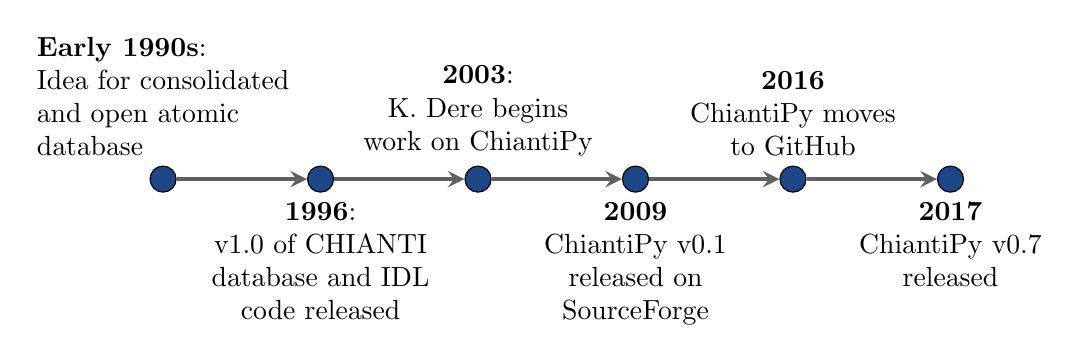
\begin{tikzpicture}[node distance=2cm]
  % Draw nodes
  \node (e1)[event,
             label={[align=left]above:\textbf{Early 1990s}:\\Idea for consolidated\\and open atomic\\database}]{};
  \node (e2)[event, right of=e1, 
             label={[align=center ]below:\textbf{1996}:\\v1.0 of CHIANTI\\database and IDL\\code released}]{};
  \node (e3)[event, right of=e2, 
             label={[align=center ]above:\textbf{2003}:\\K. Dere begins\\work on ChiantiPy}]{};
  \node (e4)[event, right of=e3,
             label={[align=center ]below:\textbf{2009}\\ChiantiPy v0.1\\released on\\SourceForge}]{};
  \node (e5)[event, right of=e4,
             label={[align=center ]above:\textbf{2016}\\ChiantiPy moves\\to GitHub}]{};
  \node (e6)[event, right of=e5,
             label={[align=center ]below:\textbf{2017}\\ChiantiPy v0.7\\released}]{};
  % Draw arrows
  \draw [arrow] (e1) -- (e2);
  \draw [arrow] (e2) -- (e3);
  \draw [arrow] (e3) -- (e4);
  \draw [arrow] (e4) -- (e5);
  \draw [arrow] (e5) -- (e6);
\end{tikzpicture}
\end{document}